\chapter{Choosing a multiplication algorithm}
\label{ch:muldispatch}

\Cref{ch:mul,ch:ntt} described four methods. This chapter explains how
\code{Multiply} picks one. The implementation is in
\file{src/algorithms/Multiplication.cpp}.

\section{The decision, step by step}

\Cref{fig:muldispatch} shows the tests in the order the code applies them. The first one
matching the operands decides; the sections after the figures explain where each number
comes from.

\begin{figure}[tbp]
\centering
\begin{tikzpicture}[node distance=6mm and 10mm]
  \node[box,fill=paper] (start) {$a \times b$ \quad ($n_a$, $n_b$ limbs)};
  \node[dec,below=of start] (small) {both $\le 16$?};
  \node[algo,fill=sAqua,right=of small] (stack) {stack-buffer\\schoolbook};
  \node[dec,below=of small] (one) {one operand\\is 1 limb?};
  \node[algo,fill=sAqua,right=of one] (mul1) {\code{Mul1}};
  \node[dec,below=of one] (sq) {same object\\and $\le 319$?};
  \node[algo,fill=sBlue,right=of sq] (sqd) {square\\dispatcher};
  \node[dec,below=of sq] (cl) {$\min \le 24$ or\\sum $\le 56$?};
  \node[algo,fill=sAqua,right=of cl] (school) {schoolbook};
  \node[dec,below=of cl] (ntt) {sum $\ge 640$, $\min \ge 64$,\\$n_a n_b \ge 96\,000$?};
  \node[algo,fill=sBlue,left=of ntt] (kar) {Karatsuba\\(+Toom-3 levels)};
  \node[dec,below=of ntt] (cold) {$n_a n_b \ge 262\,144$\\or pool awake?};
  \node[algo,fill=sOrange,right=of cold] (nttx) {NTT};
  \node[algo,fill=sBlue,left=of cold] (kar2) {Karatsuba\\(and wake pool\\if in a burst)};
  \draw[arr] (start) -- (small);
  \draw[arr] (small) -- node[above,lbl]{yes} (stack);
  \draw[arr] (small) -- node[left,lbl]{no} (one);
  \draw[arr] (one) -- node[above,lbl]{yes} (mul1);
  \draw[arr] (one) -- node[left,lbl]{no} (sq);
  \draw[arr] (sq) -- node[above,lbl]{yes} (sqd);
  \draw[arr] (sq) -- node[left,lbl]{no} (cl);
  \draw[arr] (cl) -- node[above,lbl]{yes} (school);
  \draw[arr] (cl) -- node[right,lbl]{no} (ntt);
  \draw[arr] (ntt) -- node[above,lbl]{no} (kar);
  \draw[arr] (ntt) -- node[right,lbl]{yes} (cold);
  \draw[arr] (cold) -- node[above,lbl]{yes} (nttx);
  \draw[arr] (cold) -- node[above,lbl]{no} (kar2);
\end{tikzpicture}
\caption{The multiplication dispatcher with 64-bit limbs and generic thresholds.
The stack-buffer test happens in the operator layer.}
\label{fig:muldispatch}
\end{figure}

\Cref{fig:muldispmap} draws the same rules as a map over operand shapes. Each point is a
pair of lengths; its colour is the algorithm that runs.

\begin{figure}[ht]
\centering
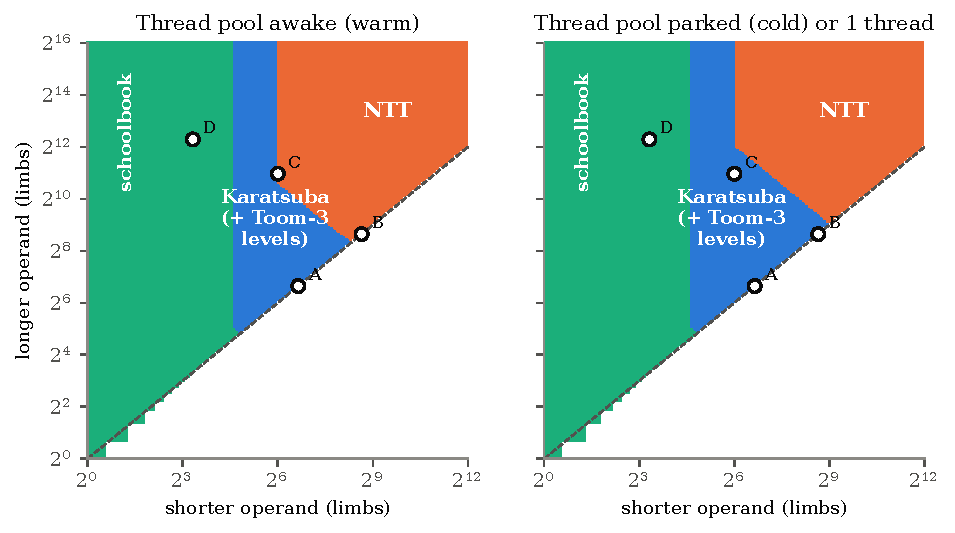
\includegraphics[width=\textwidth]{figures/mul_dispatch_map.pdf}
\caption{Which algorithm multiplies an $n_{\min} \times n_{\max}$ product, with the thread
pool awake (left) and parked or disabled (right), using the generic thresholds.
Points A--D are the worked examples in \cref{sec:mulexamples}.}
\label{fig:muldispmap}
\end{figure}

\section{Rule 1: schoolbook when the short operand is short}

Schoolbook runs when the shorter operand has at most 24 limbs, or both together have at most
56. The 24 is not a coincidence: it is the Karatsuba leaf size. If the shorter operand is
already at or below the leaf size, Karatsuba would just slice the long operand and hand every
piece to the schoolbook kernel anyway, so calling schoolbook directly skips the bookkeeping.

Note that this holds \emph{however long} the other operand is: $10 \times 100\,000$ limbs is a
schoolbook product. Its cost, $10 \times 100\,000$ limb products, is linear in the long
operand, and no fancier method can beat a single pass over the data by much.

\section{Rule 2: the NTT when the product is big \emph{in area}}
\label{sec:arearule}

For balanced products the NTT overtakes Karatsuba at about 310 limbs per operand. For
lopsided products the story is different, and this is where the shape map's slanted
boundary comes from.

Recall from \cref{sec:karatsuba} that sliced Karatsuba costs about
$n_{\max} \cdot K(n_{\min})/n_{\min}$: linear in the long operand, at a per-limb rate set by
the short one (measured 26\,ns per long-operand limb when $n_{\min} = 64$, 41\,ns at 128,
64\,ns at 256). The NTT's cost follows the \emph{total} length. So the shorter the short
operand, the longer the product must be before the NTT wins:

\begin{center}
\small
\begin{tabular}{rrr}
\toprule
shorter operand & NTT wins from (longer) & area $n_a n_b$ at crossover \\
\midrule
48 & never (at $48 \times 6144$: 139 vs 146\,\textmu s for Karatsuba) & --- \\
64 & $\approx$ 1500--2000 & 96k--128k \\
128 & $\approx$ 750 & 96k \\
160 & $\approx$ 630 & 101k \\
256 & $\approx$ 450 & 115k \\
balanced & 320 & 102k \\
\bottomrule
\end{tabular}
\end{center}

The crossover sits at a nearly constant \emph{area} $n_a \times n_b$, the number of limb
products schoolbook would need. That gives a simple rule with three conditions:
\[
n_a + n_b \ge 640, \qquad \min(n_a,n_b)\ge 64, \qquad n_a n_b \ge 96\,000.
\]
These generic floors make a product eligible for the NTT. The worker-state
rule below makes the final choice between the NTT and recursive multiplication.

\begin{another}
Think of the cost of each method as a surface over the $(n_{\min}, n_{\max})$ plane. The
dispatcher's job is to report which surface is lowest at each point. The boundaries in
\cref{fig:muldispmap} are where two surfaces cross. Measuring on a grid of shapes, not just
on balanced products, is what revealed that the Karatsuba/NTT boundary is a curve of
constant area rather than a line of constant total size.
\end{another}

\section{Rule 3: is the thread pool awake?}
\label{sec:poolrule}

The 96\,000 area threshold was measured with multiplications running back to back. In that
situation the pool's worker threads never fall asleep, and a small NTT spreads its six
transforms across six awake cores. An \emph{isolated} multiplication is different. Parked
threads take 20--30\,\textmu s to wake, which is as long as the whole product, so the
calling thread ends up doing nearly all the work itself.

\begin{figure}[ht]
\centering
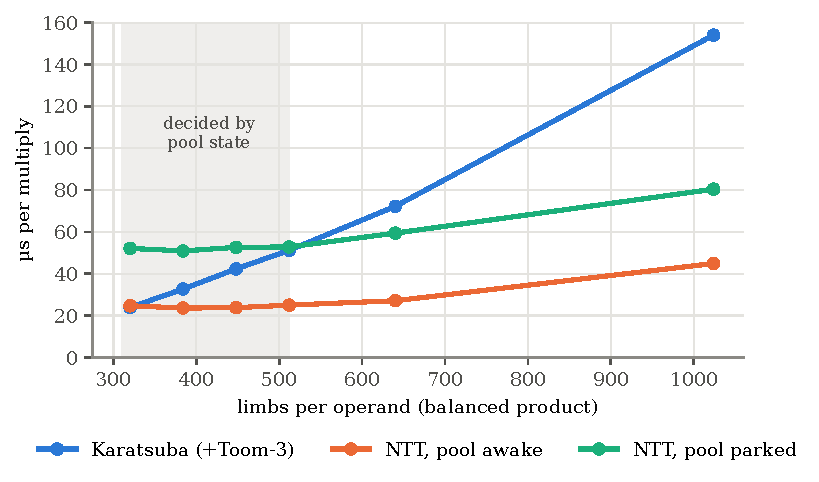
\includegraphics[width=0.8\textwidth]{figures/pool_temperature.pdf}
\caption{Time per balanced multiply. With the pool awake the NTT wins from about 320 limbs;
with the pool parked it costs about its serial time and only wins from about 512 limbs.
Data from \file{docs/MULTIPLICATION.md} (M1 Max).}
\label{fig:pool}
\end{figure}

So between area 96\,000 and 262\,144 ($\approx 512 \times 512$) the dispatcher asks the pool
whether it is awake. If yes, NTT; if not, Karatsuba. Above 262\,144 the NTT wins even cold.

There is one more twist. If a program does a \emph{burst} of mid-sized multiplications, the
first one finds the pool asleep and uses Karatsuba, which is right for it. But then every
later one would too, and the pool would never wake. To prevent this, a thread that finishes
two cold operations within 100\,\textmu s (\code{BIGMATH\_POOL\_SPIN\_US}) of each other
nudges the pool awake without giving it work. The third multiplication of the burst then
finds it warm and takes the NTT. An isolated multiplication wakes nothing.

\begin{practice}
Both paths compute the same exact product. With the generic profile,
\code{-DBIGMATH\_USE\_THREADS=0} uses the cold thresholds. The macOS Arm64
Clang profile adds a single-thread floor of 704 limbs for distinct operands
whose lengths differ by at most one limb. It leaves the threaded
worker-state rule in place.
\end{practice}

On the M1 Max, the one-thread recursive kernel took 40.0\,\textmu s
at $520\times520$ limbs, versus 46.5\,\textmu s for the NTT. At
$720\times720$, the NTT took 65.9\,\textmu s and recursion took
69.7\,\textmu s. The Apple silicon Clang kernel also specializes
schoolbook row widths from 12 through 24 limbs. Its NEON radix-8
butterflies reuse groups of twiddle factors and reduction constants
across blocks on short, repeated stages. See \file{BENCHMARK.md} for the
paired measurements through one million decimal digits.

\section{Squares}
\label{sec:sqdispatch}

When both operands are the same object (\code{x * x}) and have at most 319 limbs, the
multiplication goes straight to the square dispatcher, which exploits the symmetry of
\cref{sec:square}. Larger self-products go through the normal rules above. The ordinary
and truncated CRT transforms can reuse the spectrum of the shared operand
(\cref{sec:nttreuse}).

For a direct call to the square dispatcher, the generic thresholds are:

\begin{center}
\small
\begin{tabular}{ll}
\toprule
size (limbs) & square method \\
\midrule
1 & single-limb square \\
$< 48$ (inside Karatsuba square) & schoolbook square (\code{SqrBasecase}) \\
$48$--$351$ & Karatsuba square, Toom-3 levels from 160 \\
$352$--$607$ & NTT if the pool is awake, else Karatsuba square \\
$\ge 608$ & NTT self-product (see \cref{sec:nttreuse}) \\
\bottomrule
\end{tabular}
\end{center}

The profile can override the two NTT square floors
(\cref{sec:platformprofiles}). The ordinary CRT path saves three forward
transforms by reusing one spectrum per prime.

\section{Worked dispatch examples}
\label{sec:mulexamples}

\begin{example}[s: which algorithm runs?]
\begin{description}[leftmargin=1.2cm,style=nextline]
  \item[A: $100 \times 100$] Shorter operand $100 > 24$ and sum $200 > 56$: not schoolbook.
        Sum $200 < 640$: not NTT. $\Rightarrow$ \textbf{Karatsuba}. Its pieces (50, then 25)
        are below 168, so no Toom-3 level; the 25-limb pieces split once more to 13, which is
        under 24, so schoolbook leaves.
  \item[B: $400 \times 400$] Sum 800, minimum 400, area 160\,000: passes all three NTT tests.
        Area is below 262\,144, so it depends on the pool: \textbf{NTT} if awake (about
        24\,\textmu s), \textbf{Karatsuba} with a Toom-3 top level if parked (about 35\,\textmu s,
        better than a cold NTT's 51\,\textmu s).
  \item[C: $64 \times 2000$] Minimum 64 passes, sum 2064 passes, area 128\,000 passes.
        Warm: \textbf{NTT}. Cold: \textbf{Karatsuba}, slicing the long operand into 32 balanced
        $64 \times 64$ products.
  \item[D: $10 \times 5000$] Shorter operand $10 \le 24$: \textbf{schoolbook}, ten
        \code{AddMul1} rows over 5000 limbs.
  \item[E: $600 \times 600$] Area 360\,000 $\ge$ 262\,144: \textbf{NTT} regardless of the pool.
        The product has $2 \cdot 2 \cdot 600 = 2400$ coefficients, just above $H = 2048$, so the
        $H + L$ scheme runs with $L = 512$: transform work 2560 instead of 4096.
\end{description}
\end{example}

\section{How the rules were found}

The generic thresholds were re-measured on 20--21 November 2026, after the limb kernels,
Karatsuba slicing, and NTT improvements had all moved the crossovers. The procedure:
time every algorithm directly on a grid of shapes ($n_{\min}$ from 8 to 256 limbs,
ratios 1 to 128), find where each pair crosses, and fit the simplest rule that matches.
After the change the largest remaining mis-routes were near-ties within 17\% of the best
method.

\begin{perfnote}
End-to-end effect of that re-sweep, through the public API (M1 Max, warm):
multiplying two 20\,000-digit numbers went from 0.219\,ms to 0.048\,ms (4.6$\times$), and
from 2.7 times GMP's time to 0.6 times. 1\,000\,000-digit parsing and printing became
1.8 times faster without any change to their own code, because they are built on
\code{Multiply}.
\end{perfnote}
